\section{SIMD and vector}
    We already introduce SIMD in the \hyperlink{simd}{\textbf{section 2.1}}. In the basic scalar pipeline, execution is in one simple ALU, and this code 
    \hypertarget{daxpy}{}
    \begin{codeCenter}
    \begin{Ccode}
void daxpy(int n, double a, double* x, double* y){
    for(int i = 0; 0 < n; i++){
        y[i] = a * x[i] + y[i];
    }           
}
    \end{Ccode}
    \end{codeCenter}
    would look like this:
    \begin{codeCenter}
    \begin{Ccode}
loop:
    lw r1, 0(r2) //load x[i]
    lw r6, 0(r3) //load y[i]
    mul r1, r1, r4  //a*x[i]
    add r6, r1, r6  //... + y[i]
    sw r6, 0(r3)  //store y[i]
    add r2, r2, 8
    add r3, r3, 8
    bne r2, r5, loop
    \end{Ccode}
    \end{codeCenter}
    \begin{tcolorbox}[gris]
        If we are doing 1024 iterations, we'll have $8 \cdot 1024 = 8192$ instructions. \\
        We can count the number of misses too, a size of double is 8B, a cache line 64B $\implies$ 8 elements per block. We have two loads by loop, then we know that we have $\frac{2\cdot 1024}{8}=256$ misses.
    \end{tcolorbox}
    If we want to optimize this by having a out-of-order processor and a re-order buffer (c.f. computer architecture), knowing that a ROB is of size $\approx 500$ instructions, it is only 6\% of instructions that can be in the ROB. We can't augment the ROB size because it adds too much overhead $\implies$ out-of-order processors are not a very good solution.
    \newpage
    Let's introduce vector pipeline:
    \begin{center}
        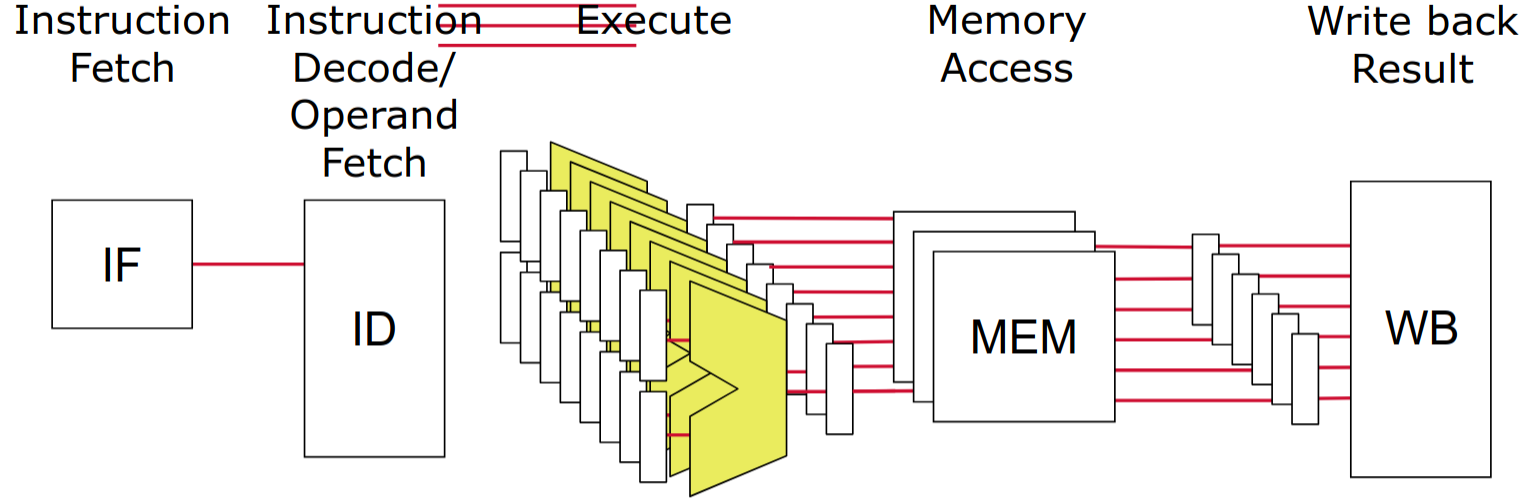
\includegraphics[width=9cm]{images/20.png}
    \end{center}
    \begin{tcolorbox}[rouge]
        The vector processors:
        \begin{itemize}[left=10pt, label=\textbullet]
            \item Reduces instruction bloat, 
            \item Simplifies dependency checking, 
            \item Potentially reduce cache misses, 
            \item Reduces control hazards.
        \end{itemize}
    \end{tcolorbox}
    \begin{tcolorbox}[gris]
        \textbf{Examples of vector instructions:}
        \begin{itemize}[left=10pt, label=\textbullet]
            \item \lstinline!mul.v v1, v2, v1! does the dot product v1 $\cdot$ v2.
            \item  \lstinline!mul.sv v1, r2, v1! multiplies scalar r1 to all elements of v1. 
            \item \lstinline!lw.v v1, O(r1)! loads vector v1 from address r1. 
            \item \lstinline!sw.v v1, O(r1)! stores vector v1 at address r1.
        \end{itemize}
    \end{tcolorbox}
    Then our compiler code would look like this:
    \begin{codeCenter}
    \begin{Ccode}
loop:
    lw.v v1, 0(r2) ; load x[i]
    lw.v v2, 0(r3) ; load y[i]
    mul.sv v1, r4, v1 ; a*x[i]
    add.v v1, v1, v2 ; … + y[i]
    sw.v v1, 0(r3) ; store y[i]
    add r2, r2, 512 ; 64*8
    add r3, r3, 512
    bne r2, r5, loop
    \end{Ccode}
    \end{codeCenter}
    \begin{tcolorbox}[gris]
        Now for 1024 iterations of our loop, we only have $8\cdot \left(\frac{1024}{64}\right)=128$ instructions. For misses, the vector load brings 64 elements at a time $\implies$ 8 cache lines $\implies 2\cdot \left(\frac{1024}{64}\right)=32$.
    \end{tcolorbox}
    To apply SIMD we need a specific hardware: 
    \begin{itemize}[left=10pt, label=\textbullet]
        \item Vector registers to store multiple elements of a vector in a single register, 
        \item Replicated functional units inside the pipeline of a core (multiple lane/ALUs), 
        \item Support for decoding new instructions (SIMD instructions).
    \end{itemize}
    \subsection{AVX instructions}
        
    AVX instructions are for 256-bit operations on x86 architecture.
    \begin{center}
    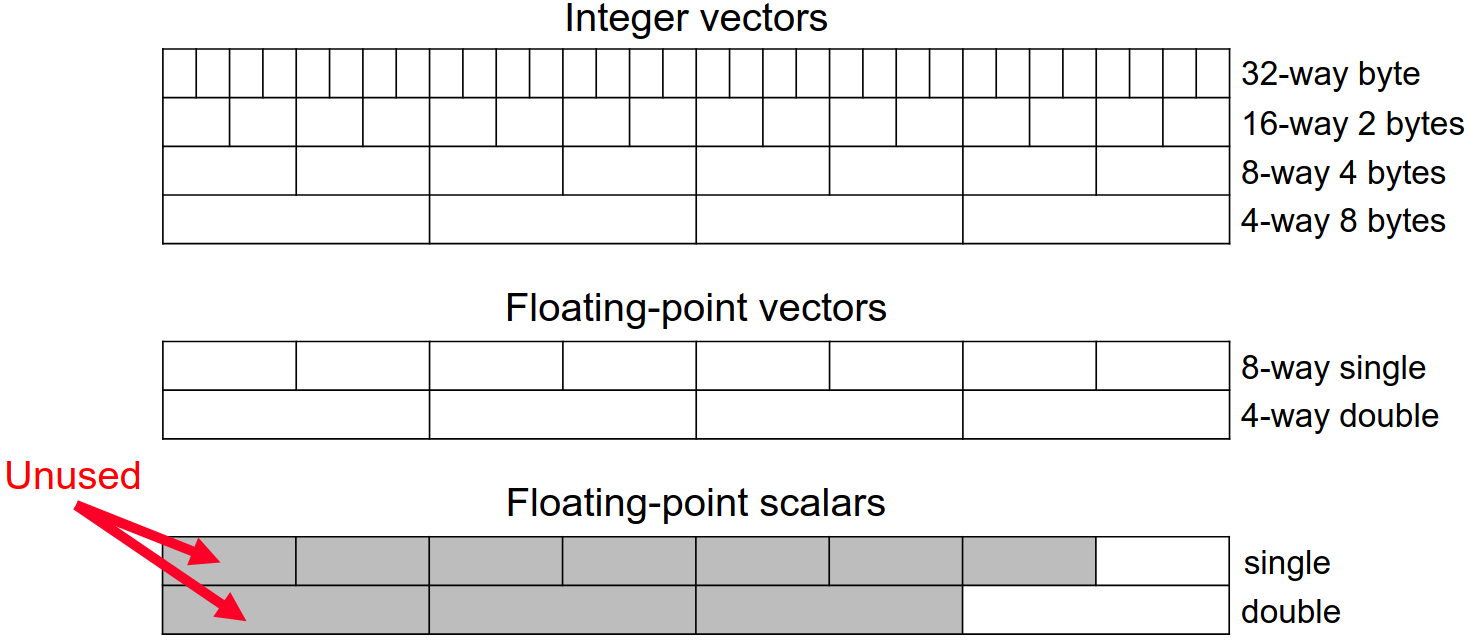
\includegraphics[width=10cm]{images/21.png}
    \end{center}
    \begin{tcolorbox}[violet]
    Let's interpret an AVX instructions e.g. \lstinline!vaddpd!:
    \begin{itemize}[left=10pt, label=\textbullet]
        \item \lstinline!v! means that is an AVX instructions,
        \item \lstinline!add! indicate the operation,
        \item \lstinline!p! means packed, it can also be \lstinline!s!, then it would be scalar (you can see upper),
        \item \lstinline!d! stand for double-precision, can be \lstinline!s! for single-precision, etc\ldots
    \end{itemize}
    \end{tcolorbox}
    To use AVX instructions there is multiple way, the simplest is to auto-compile the code by using -O3 when compiling C code. But there is two main problems with the auto-compile solution. Aliasing and alignment.\\
    \begin{tcolorbox}[vert]
       \important{Aliasing:} 

        Let's take again our \hyperlink{daxpy}{\textbf{daxpy}} code, the compiler can't say at 100\% that pointers are independent, then it won't vectorize. To solve this we have to say to the compiler that pointers don't overlap by changing the signature into
        \begin{codeCenter}
        \begin{Ccode}
void daxpy(int n, double a, double* restrict x, double* restrict y);
        \end{Ccode}
        \end{codeCenter}
    \end{tcolorbox}
    \begin{tcolorbox}[vert]
        \important{Alignment:}

        Modern DRAM accesses are per four bytes and for better performances, accesses to vector elements should be aligned.     
    \end{tcolorbox}
    for example, to load an 8-element 32-bit vector:
    \begin{center}
    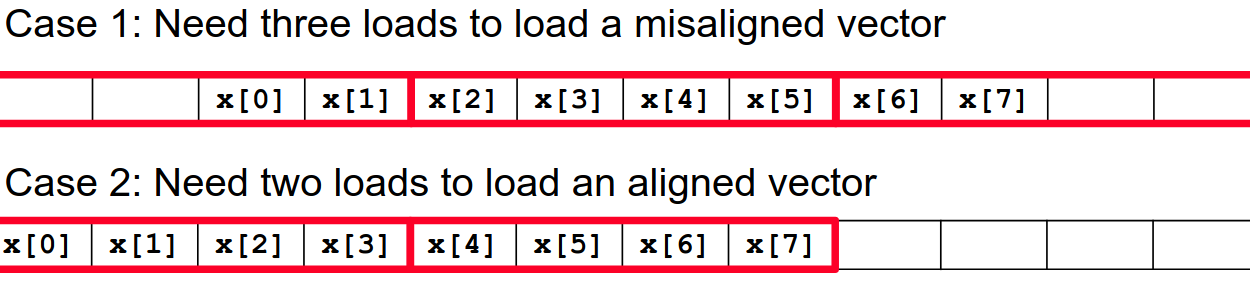
\includegraphics[width=10cm]{images/22.png}
    \end{center}
    To solve this, you can use \lstinline!aligned_alloc! in C when allocating arrays and \lstinline!_attribute_((aligned(32)))! for static arrays.
    \begin{tcolorbox}[rouge]
        To summarize, the compiler cannot vectorize if:
        \begin{itemize}[left=10pt, label=\textbullet]
            \item There is loop with unknown number of iterations at runtime,
            \item There is if-else statements or diverging condition inside loop,
            \item There is dependence between loop iterations, 
            \item There is function calls in the loop body.
        \end{itemize}
    \end{tcolorbox}

    Another way to use AVX instructions is to optimize the code manually with ``intrisics''. Intrisics are compiler-provided functions that map directly to specific CPU instructions.
    \begin{image}{Different intrisics data types }
        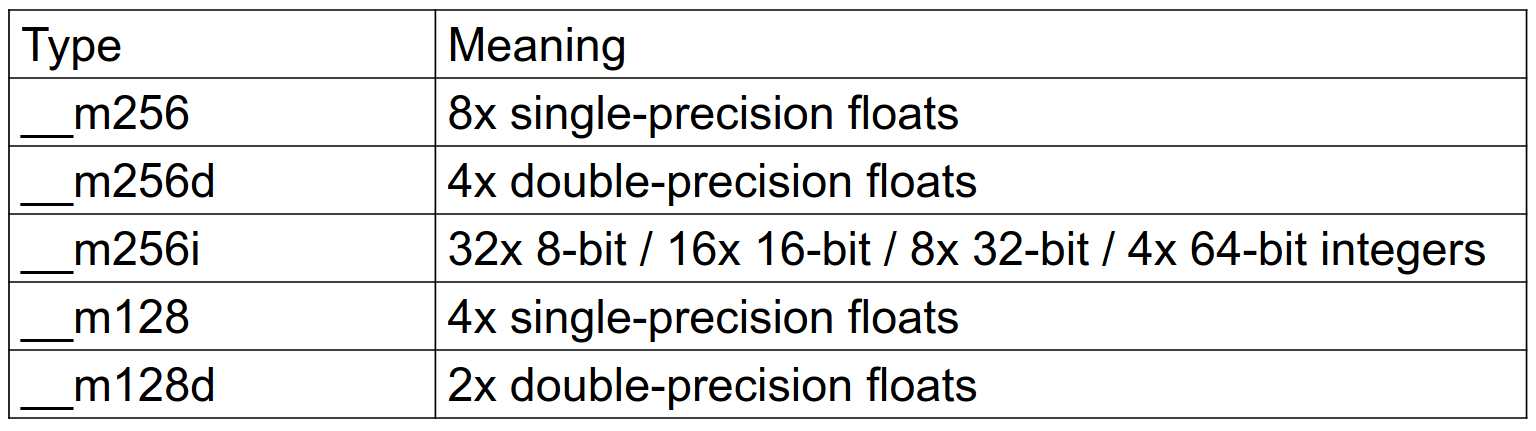
\includegraphics[width=9cm]{images/23.png}
    \end{image}
    \begin{tcolorbox}[violet]
        Let's interpret an AVX intrisics function e.g. \\
        \lstinline!_mm256_op_suffix(type param1, type param2, type param3)!:
        \begin{itemize}[left=10pt, label=\textbullet]
            \item \lstinline!mm256! means that we are working on the 256-bit registers,
            \item \lstinline!op! is the operation to do, e.g. add, sub, load, etc\ldots
            \item \lstinline!suffix! is the type of the returned vector, e.g. ps, pd, epi32, epu64, etc\ldots
        \end{itemize}
    \end{tcolorbox}
    With this, our \hyperlink{daxpy}{\textbf{daxpy}} code would become 
    \begin{codeCenter}
    \begin{Ccode}
__m256d vecA = _mm256_set_pd(a, a, a, a);

for(int i = 0; i < n; i+=4) {
    __m256d vecX = _mm256_load_pd(&x[i]); //Load x[i]...
    __m256d vecY = _mm256_load_pd(&y[i]); //Load y[i]...
    __m256d vecZ = _mm256_mul_pd(vecA, vecX); //  a*x
    
    vecY = _mm256_add_pd(vecZ, vecY); // ... + y
    
    // Store result back to y
    _mm256_store_pd(&y[i], vecY);
}
    \end{Ccode}
    \end{codeCenter}
    AVX intrinsic C code optimize a lot normal code because cache misses are optimized too.
